\section{Analisi dati}
\label{analisiDati}

\subsection{Script}

In questo progetto sono presenti 2 script in linguaggio R con lo scopo di popolare la base di dati e generare i grafici presenti qui sotto.

Lo script R/popolamento.r si occupa di generare dati casuali per ognuna delle 4 tabelle del database con il volume specificato nella \hyperref[tabellaValori]{Tabella valori} e successivamente di inserirli nel database.

Lo script R/grafici.r preleva i dati dal database, li analizza e genera gli 11 grafici presenti qui sotto.

\subsection{Grafici}

\begin{figure}[h]
	\caption{Grafico 1}
	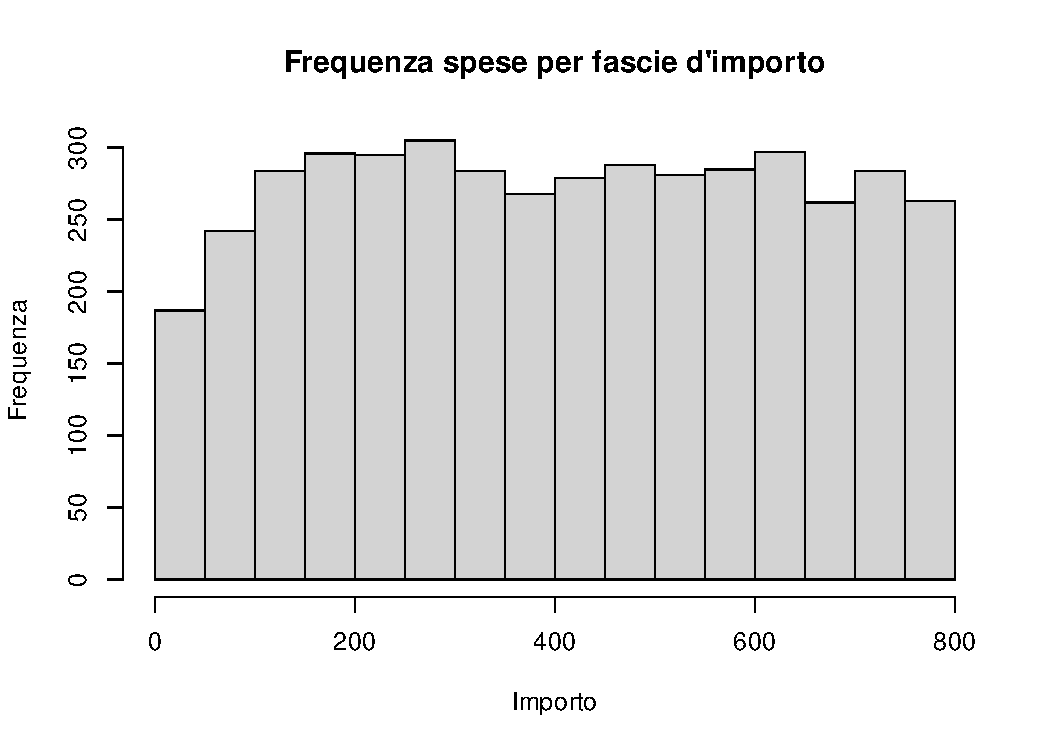
\includegraphics[page=1,width=\textwidth]{../R/grafici.pdf}
	\label{fig1}
\end{figure}

Primo grafico in figura \ref{fig1}. \textbf{Osservazioni}: Il grafico mostra come le spese siano distribuite in diverse fasce d'importo, con una distribuzione uniforme ma con alcune leggere variazioni nella frequenza. Si può notare in particolare che la fascia d'importo tra 0 e 200 sembra avere una frequenza leggermente inferiore rispetto alle altre fasce.

\clearpage

\begin{figure}[h]
    \centering
    \begin{subfigure}[b]{0.5\textwidth}
        \centering
        \includegraphics[page=2,width=\textwidth]{../R/grafici.pdf}
    \end{subfigure}
    \hfill
    \begin{subfigure}[b]{0.5\textwidth}
        \centering
        \includegraphics[page=3,width=\textwidth]{../R/grafici.pdf}
    \end{subfigure}
    \caption{Grafico 2 e 3}
    \label{fig2}
\end{figure}

Secondo e terzo grafico in figura \ref{fig2}. \textbf{Osservazioni}: Il grafico mostra la relazione tra il numero di appartamenti e l'ammontare complessivo delle spese nei condomini. Si nota un trend in cui l'ammontare complessivo tende ad aumentare con il numero di appartamenti.

\clearpage

\begin{figure}[t]
	\caption{Grafico 4}
	\includegraphics[page=4,width=\textwidth]{../R/grafici.pdf}
	\label{fig3}
\end{figure}

Quarto grafico in figura \ref{fig3}. \textbf{Osservazioni}: Questo grafico evidenzia come la quota dell'anno corrente varia in relazione alla superficie degli appartamenti. Solitamente, una superficie maggiore comporta una quota annuale maggiore.

\clearpage

\begin{figure}[t]
	\caption{Grafico 5}
	\includegraphics[page=5,width=\textwidth]{../R/grafici.pdf}
	\label{fig5}
\end{figure}

Quinto grafico in figura \ref{fig5}. \textbf{Osservazioni}: Simile al grafico precedente, questo grafico mostra la relazione inversa, ovvero come la superficie varia in funzione della quota anno corrente.


\clearpage

\begin{figure}[t]
	\caption{Grafico 6}
	\includegraphics[page=6,width=\textwidth]{../R/grafici.pdf}
	\label{fig6}
\end{figure}

Sesto grafico in figura \ref{fig6}. \textbf{Osservazioni}: Questo grafico illustra la distribuzione della superficie degli appartamenti di un singolo condominio random. Mostra la frequenza delle superfici degli appartamenti all'interno di un dato condominio.


\clearpage

\begin{figure}[t]
	\caption{Grafico 7}
	\includegraphics[page=7,width=\textwidth]{../R/grafici.pdf}
	\label{fig7}
\end{figure}

Settimo grafico in figura \ref{fig7}. \textbf{Osservazioni}: Simile al grafico precedente, ma per un campione più grande di condomini. Mostra la frequenza delle superfici di tutti gli appartamenti del sistema.


\clearpage

\begin{figure}[t]
	\caption{Grafico 8}
	\includegraphics[page=8,width=\textwidth]{../R/grafici.pdf}
	\label{fig8}
\end{figure}

Ottavo grafico in figura \ref{fig8}. \textbf{Osservazioni}: Il grafico mostra come la percentuale di spese pagate è distribuita tra gli appartamenti.

\clearpage

\begin{figure}[t]
	\caption{Grafico 9}
	\includegraphics[page=9,width=\textwidth]{../R/grafici.pdf}
	\label{fig9}
\end{figure}


Nono grafico in figura \ref{fig9}. \textbf{Osservazioni}: Questo grafico evidenzia la relazione tra la superficie degli appartamenti e quanto effettivamente pagato rispetto alla quota annuale corrente. Può rivelare se appartamenti più grandi tendono a pagare più o meno rispetto alla quota prevista.

\clearpage

\begin{figure}[t]
	\caption{Grafico 10}
	\includegraphics[page=10,width=\textwidth]{../R/grafici.pdf}
	\label{fig10}
\end{figure}

Decimo grafico in figura \ref{fig10}. \textbf{Osservazioni}: Questo grafico mostra come le spese sono distribuite tra le varie causali in un singolo condominio random. Le categorie con percentuali più elevate rappresentano le spese maggiori.

\clearpage

\begin{figure}[t]
	\caption{Grafico 11}
	\includegraphics[page=11,width=\textwidth]{../R/grafici.pdf}
	\label{fig11}
\end{figure}

Undicesimo grafico in figura \ref{fig11}. Come il grafico precedente ma prendendo in considerazione tutti i condomini del sistema.
